
% Default to the notebook output style

    


% Inherit from the specified cell style.




    
\documentclass[11pt]{article}

    
    
    \usepackage[T1]{fontenc}
    % Nicer default font (+ math font) than Computer Modern for most use cases
    \usepackage{mathpazo}

    % Basic figure setup, for now with no caption control since it's done
    % automatically by Pandoc (which extracts ![](path) syntax from Markdown).
    \usepackage{graphicx}
    % We will generate all images so they have a width \maxwidth. This means
    % that they will get their normal width if they fit onto the page, but
    % are scaled down if they would overflow the margins.
    \makeatletter
    \def\maxwidth{\ifdim\Gin@nat@width>\linewidth\linewidth
    \else\Gin@nat@width\fi}
    \makeatother
    \let\Oldincludegraphics\includegraphics
    % Set max figure width to be 80% of text width, for now hardcoded.
    \renewcommand{\includegraphics}[1]{\Oldincludegraphics[width=.8\maxwidth]{#1}}
    % Ensure that by default, figures have no caption (until we provide a
    % proper Figure object with a Caption API and a way to capture that
    % in the conversion process - todo).
    \usepackage{caption}
    \DeclareCaptionLabelFormat{nolabel}{}
    \captionsetup{labelformat=nolabel}

    \usepackage{adjustbox} % Used to constrain images to a maximum size 
    \usepackage{xcolor} % Allow colors to be defined
    \usepackage{enumerate} % Needed for markdown enumerations to work
    \usepackage{geometry} % Used to adjust the document margins
    \usepackage{amsmath} % Equations
    \usepackage{amssymb} % Equations
    \usepackage{textcomp} % defines textquotesingle
    % Hack from http://tex.stackexchange.com/a/47451/13684:
    \AtBeginDocument{%
        \def\PYZsq{\textquotesingle}% Upright quotes in Pygmentized code
    }
    \usepackage{upquote} % Upright quotes for verbatim code
    \usepackage{eurosym} % defines \euro
    \usepackage[mathletters]{ucs} % Extended unicode (utf-8) support
    \usepackage[utf8x]{inputenc} % Allow utf-8 characters in the tex document
    \usepackage{fancyvrb} % verbatim replacement that allows latex
    \usepackage{grffile} % extends the file name processing of package graphics 
                         % to support a larger range 
    % The hyperref package gives us a pdf with properly built
    % internal navigation ('pdf bookmarks' for the table of contents,
    % internal cross-reference links, web links for URLs, etc.)
    \usepackage{hyperref}
    \usepackage{longtable} % longtable support required by pandoc >1.10
    \usepackage{booktabs}  % table support for pandoc > 1.12.2
    \usepackage[inline]{enumitem} % IRkernel/repr support (it uses the enumerate* environment)
    \usepackage[normalem]{ulem} % ulem is needed to support strikethroughs (\sout)
                                % normalem makes italics be italics, not underlines
    

    
    
    % Colors for the hyperref package
    \definecolor{urlcolor}{rgb}{0,.145,.698}
    \definecolor{linkcolor}{rgb}{.71,0.21,0.01}
    \definecolor{citecolor}{rgb}{.12,.54,.11}

    % ANSI colors
    \definecolor{ansi-black}{HTML}{3E424D}
    \definecolor{ansi-black-intense}{HTML}{282C36}
    \definecolor{ansi-red}{HTML}{E75C58}
    \definecolor{ansi-red-intense}{HTML}{B22B31}
    \definecolor{ansi-green}{HTML}{00A250}
    \definecolor{ansi-green-intense}{HTML}{007427}
    \definecolor{ansi-yellow}{HTML}{DDB62B}
    \definecolor{ansi-yellow-intense}{HTML}{B27D12}
    \definecolor{ansi-blue}{HTML}{208FFB}
    \definecolor{ansi-blue-intense}{HTML}{0065CA}
    \definecolor{ansi-magenta}{HTML}{D160C4}
    \definecolor{ansi-magenta-intense}{HTML}{A03196}
    \definecolor{ansi-cyan}{HTML}{60C6C8}
    \definecolor{ansi-cyan-intense}{HTML}{258F8F}
    \definecolor{ansi-white}{HTML}{C5C1B4}
    \definecolor{ansi-white-intense}{HTML}{A1A6B2}

    % commands and environments needed by pandoc snippets
    % extracted from the output of `pandoc -s`
    \providecommand{\tightlist}{%
      \setlength{\itemsep}{0pt}\setlength{\parskip}{0pt}}
    \DefineVerbatimEnvironment{Highlighting}{Verbatim}{commandchars=\\\{\}}
    % Add ',fontsize=\small' for more characters per line
    \newenvironment{Shaded}{}{}
    \newcommand{\KeywordTok}[1]{\textcolor[rgb]{0.00,0.44,0.13}{\textbf{{#1}}}}
    \newcommand{\DataTypeTok}[1]{\textcolor[rgb]{0.56,0.13,0.00}{{#1}}}
    \newcommand{\DecValTok}[1]{\textcolor[rgb]{0.25,0.63,0.44}{{#1}}}
    \newcommand{\BaseNTok}[1]{\textcolor[rgb]{0.25,0.63,0.44}{{#1}}}
    \newcommand{\FloatTok}[1]{\textcolor[rgb]{0.25,0.63,0.44}{{#1}}}
    \newcommand{\CharTok}[1]{\textcolor[rgb]{0.25,0.44,0.63}{{#1}}}
    \newcommand{\StringTok}[1]{\textcolor[rgb]{0.25,0.44,0.63}{{#1}}}
    \newcommand{\CommentTok}[1]{\textcolor[rgb]{0.38,0.63,0.69}{\textit{{#1}}}}
    \newcommand{\OtherTok}[1]{\textcolor[rgb]{0.00,0.44,0.13}{{#1}}}
    \newcommand{\AlertTok}[1]{\textcolor[rgb]{1.00,0.00,0.00}{\textbf{{#1}}}}
    \newcommand{\FunctionTok}[1]{\textcolor[rgb]{0.02,0.16,0.49}{{#1}}}
    \newcommand{\RegionMarkerTok}[1]{{#1}}
    \newcommand{\ErrorTok}[1]{\textcolor[rgb]{1.00,0.00,0.00}{\textbf{{#1}}}}
    \newcommand{\NormalTok}[1]{{#1}}
    
    % Additional commands for more recent versions of Pandoc
    \newcommand{\ConstantTok}[1]{\textcolor[rgb]{0.53,0.00,0.00}{{#1}}}
    \newcommand{\SpecialCharTok}[1]{\textcolor[rgb]{0.25,0.44,0.63}{{#1}}}
    \newcommand{\VerbatimStringTok}[1]{\textcolor[rgb]{0.25,0.44,0.63}{{#1}}}
    \newcommand{\SpecialStringTok}[1]{\textcolor[rgb]{0.73,0.40,0.53}{{#1}}}
    \newcommand{\ImportTok}[1]{{#1}}
    \newcommand{\DocumentationTok}[1]{\textcolor[rgb]{0.73,0.13,0.13}{\textit{{#1}}}}
    \newcommand{\AnnotationTok}[1]{\textcolor[rgb]{0.38,0.63,0.69}{\textbf{\textit{{#1}}}}}
    \newcommand{\CommentVarTok}[1]{\textcolor[rgb]{0.38,0.63,0.69}{\textbf{\textit{{#1}}}}}
    \newcommand{\VariableTok}[1]{\textcolor[rgb]{0.10,0.09,0.49}{{#1}}}
    \newcommand{\ControlFlowTok}[1]{\textcolor[rgb]{0.00,0.44,0.13}{\textbf{{#1}}}}
    \newcommand{\OperatorTok}[1]{\textcolor[rgb]{0.40,0.40,0.40}{{#1}}}
    \newcommand{\BuiltInTok}[1]{{#1}}
    \newcommand{\ExtensionTok}[1]{{#1}}
    \newcommand{\PreprocessorTok}[1]{\textcolor[rgb]{0.74,0.48,0.00}{{#1}}}
    \newcommand{\AttributeTok}[1]{\textcolor[rgb]{0.49,0.56,0.16}{{#1}}}
    \newcommand{\InformationTok}[1]{\textcolor[rgb]{0.38,0.63,0.69}{\textbf{\textit{{#1}}}}}
    \newcommand{\WarningTok}[1]{\textcolor[rgb]{0.38,0.63,0.69}{\textbf{\textit{{#1}}}}}
    
    
    % Define a nice break command that doesn't care if a line doesn't already
    % exist.
    \def\br{\hspace*{\fill} \\* }
    % Math Jax compatability definitions
    \def\gt{>}
    \def\lt{<}
    % Document parameters
    \title{ECCO\_v4\_Improving\_the\_GRID\_Dataset\_Object}
    
    
    

    % Pygments definitions
    
\makeatletter
\def\PY@reset{\let\PY@it=\relax \let\PY@bf=\relax%
    \let\PY@ul=\relax \let\PY@tc=\relax%
    \let\PY@bc=\relax \let\PY@ff=\relax}
\def\PY@tok#1{\csname PY@tok@#1\endcsname}
\def\PY@toks#1+{\ifx\relax#1\empty\else%
    \PY@tok{#1}\expandafter\PY@toks\fi}
\def\PY@do#1{\PY@bc{\PY@tc{\PY@ul{%
    \PY@it{\PY@bf{\PY@ff{#1}}}}}}}
\def\PY#1#2{\PY@reset\PY@toks#1+\relax+\PY@do{#2}}

\expandafter\def\csname PY@tok@gd\endcsname{\def\PY@tc##1{\textcolor[rgb]{0.63,0.00,0.00}{##1}}}
\expandafter\def\csname PY@tok@gu\endcsname{\let\PY@bf=\textbf\def\PY@tc##1{\textcolor[rgb]{0.50,0.00,0.50}{##1}}}
\expandafter\def\csname PY@tok@gt\endcsname{\def\PY@tc##1{\textcolor[rgb]{0.00,0.27,0.87}{##1}}}
\expandafter\def\csname PY@tok@gs\endcsname{\let\PY@bf=\textbf}
\expandafter\def\csname PY@tok@gr\endcsname{\def\PY@tc##1{\textcolor[rgb]{1.00,0.00,0.00}{##1}}}
\expandafter\def\csname PY@tok@cm\endcsname{\let\PY@it=\textit\def\PY@tc##1{\textcolor[rgb]{0.25,0.50,0.50}{##1}}}
\expandafter\def\csname PY@tok@vg\endcsname{\def\PY@tc##1{\textcolor[rgb]{0.10,0.09,0.49}{##1}}}
\expandafter\def\csname PY@tok@vi\endcsname{\def\PY@tc##1{\textcolor[rgb]{0.10,0.09,0.49}{##1}}}
\expandafter\def\csname PY@tok@vm\endcsname{\def\PY@tc##1{\textcolor[rgb]{0.10,0.09,0.49}{##1}}}
\expandafter\def\csname PY@tok@mh\endcsname{\def\PY@tc##1{\textcolor[rgb]{0.40,0.40,0.40}{##1}}}
\expandafter\def\csname PY@tok@cs\endcsname{\let\PY@it=\textit\def\PY@tc##1{\textcolor[rgb]{0.25,0.50,0.50}{##1}}}
\expandafter\def\csname PY@tok@ge\endcsname{\let\PY@it=\textit}
\expandafter\def\csname PY@tok@vc\endcsname{\def\PY@tc##1{\textcolor[rgb]{0.10,0.09,0.49}{##1}}}
\expandafter\def\csname PY@tok@il\endcsname{\def\PY@tc##1{\textcolor[rgb]{0.40,0.40,0.40}{##1}}}
\expandafter\def\csname PY@tok@go\endcsname{\def\PY@tc##1{\textcolor[rgb]{0.53,0.53,0.53}{##1}}}
\expandafter\def\csname PY@tok@cp\endcsname{\def\PY@tc##1{\textcolor[rgb]{0.74,0.48,0.00}{##1}}}
\expandafter\def\csname PY@tok@gi\endcsname{\def\PY@tc##1{\textcolor[rgb]{0.00,0.63,0.00}{##1}}}
\expandafter\def\csname PY@tok@gh\endcsname{\let\PY@bf=\textbf\def\PY@tc##1{\textcolor[rgb]{0.00,0.00,0.50}{##1}}}
\expandafter\def\csname PY@tok@ni\endcsname{\let\PY@bf=\textbf\def\PY@tc##1{\textcolor[rgb]{0.60,0.60,0.60}{##1}}}
\expandafter\def\csname PY@tok@nl\endcsname{\def\PY@tc##1{\textcolor[rgb]{0.63,0.63,0.00}{##1}}}
\expandafter\def\csname PY@tok@nn\endcsname{\let\PY@bf=\textbf\def\PY@tc##1{\textcolor[rgb]{0.00,0.00,1.00}{##1}}}
\expandafter\def\csname PY@tok@no\endcsname{\def\PY@tc##1{\textcolor[rgb]{0.53,0.00,0.00}{##1}}}
\expandafter\def\csname PY@tok@na\endcsname{\def\PY@tc##1{\textcolor[rgb]{0.49,0.56,0.16}{##1}}}
\expandafter\def\csname PY@tok@nb\endcsname{\def\PY@tc##1{\textcolor[rgb]{0.00,0.50,0.00}{##1}}}
\expandafter\def\csname PY@tok@nc\endcsname{\let\PY@bf=\textbf\def\PY@tc##1{\textcolor[rgb]{0.00,0.00,1.00}{##1}}}
\expandafter\def\csname PY@tok@nd\endcsname{\def\PY@tc##1{\textcolor[rgb]{0.67,0.13,1.00}{##1}}}
\expandafter\def\csname PY@tok@ne\endcsname{\let\PY@bf=\textbf\def\PY@tc##1{\textcolor[rgb]{0.82,0.25,0.23}{##1}}}
\expandafter\def\csname PY@tok@nf\endcsname{\def\PY@tc##1{\textcolor[rgb]{0.00,0.00,1.00}{##1}}}
\expandafter\def\csname PY@tok@si\endcsname{\let\PY@bf=\textbf\def\PY@tc##1{\textcolor[rgb]{0.73,0.40,0.53}{##1}}}
\expandafter\def\csname PY@tok@s2\endcsname{\def\PY@tc##1{\textcolor[rgb]{0.73,0.13,0.13}{##1}}}
\expandafter\def\csname PY@tok@nt\endcsname{\let\PY@bf=\textbf\def\PY@tc##1{\textcolor[rgb]{0.00,0.50,0.00}{##1}}}
\expandafter\def\csname PY@tok@nv\endcsname{\def\PY@tc##1{\textcolor[rgb]{0.10,0.09,0.49}{##1}}}
\expandafter\def\csname PY@tok@s1\endcsname{\def\PY@tc##1{\textcolor[rgb]{0.73,0.13,0.13}{##1}}}
\expandafter\def\csname PY@tok@dl\endcsname{\def\PY@tc##1{\textcolor[rgb]{0.73,0.13,0.13}{##1}}}
\expandafter\def\csname PY@tok@ch\endcsname{\let\PY@it=\textit\def\PY@tc##1{\textcolor[rgb]{0.25,0.50,0.50}{##1}}}
\expandafter\def\csname PY@tok@m\endcsname{\def\PY@tc##1{\textcolor[rgb]{0.40,0.40,0.40}{##1}}}
\expandafter\def\csname PY@tok@gp\endcsname{\let\PY@bf=\textbf\def\PY@tc##1{\textcolor[rgb]{0.00,0.00,0.50}{##1}}}
\expandafter\def\csname PY@tok@sh\endcsname{\def\PY@tc##1{\textcolor[rgb]{0.73,0.13,0.13}{##1}}}
\expandafter\def\csname PY@tok@ow\endcsname{\let\PY@bf=\textbf\def\PY@tc##1{\textcolor[rgb]{0.67,0.13,1.00}{##1}}}
\expandafter\def\csname PY@tok@sx\endcsname{\def\PY@tc##1{\textcolor[rgb]{0.00,0.50,0.00}{##1}}}
\expandafter\def\csname PY@tok@bp\endcsname{\def\PY@tc##1{\textcolor[rgb]{0.00,0.50,0.00}{##1}}}
\expandafter\def\csname PY@tok@c1\endcsname{\let\PY@it=\textit\def\PY@tc##1{\textcolor[rgb]{0.25,0.50,0.50}{##1}}}
\expandafter\def\csname PY@tok@fm\endcsname{\def\PY@tc##1{\textcolor[rgb]{0.00,0.00,1.00}{##1}}}
\expandafter\def\csname PY@tok@o\endcsname{\def\PY@tc##1{\textcolor[rgb]{0.40,0.40,0.40}{##1}}}
\expandafter\def\csname PY@tok@kc\endcsname{\let\PY@bf=\textbf\def\PY@tc##1{\textcolor[rgb]{0.00,0.50,0.00}{##1}}}
\expandafter\def\csname PY@tok@c\endcsname{\let\PY@it=\textit\def\PY@tc##1{\textcolor[rgb]{0.25,0.50,0.50}{##1}}}
\expandafter\def\csname PY@tok@mf\endcsname{\def\PY@tc##1{\textcolor[rgb]{0.40,0.40,0.40}{##1}}}
\expandafter\def\csname PY@tok@err\endcsname{\def\PY@bc##1{\setlength{\fboxsep}{0pt}\fcolorbox[rgb]{1.00,0.00,0.00}{1,1,1}{\strut ##1}}}
\expandafter\def\csname PY@tok@mb\endcsname{\def\PY@tc##1{\textcolor[rgb]{0.40,0.40,0.40}{##1}}}
\expandafter\def\csname PY@tok@ss\endcsname{\def\PY@tc##1{\textcolor[rgb]{0.10,0.09,0.49}{##1}}}
\expandafter\def\csname PY@tok@sr\endcsname{\def\PY@tc##1{\textcolor[rgb]{0.73,0.40,0.53}{##1}}}
\expandafter\def\csname PY@tok@mo\endcsname{\def\PY@tc##1{\textcolor[rgb]{0.40,0.40,0.40}{##1}}}
\expandafter\def\csname PY@tok@kd\endcsname{\let\PY@bf=\textbf\def\PY@tc##1{\textcolor[rgb]{0.00,0.50,0.00}{##1}}}
\expandafter\def\csname PY@tok@mi\endcsname{\def\PY@tc##1{\textcolor[rgb]{0.40,0.40,0.40}{##1}}}
\expandafter\def\csname PY@tok@kn\endcsname{\let\PY@bf=\textbf\def\PY@tc##1{\textcolor[rgb]{0.00,0.50,0.00}{##1}}}
\expandafter\def\csname PY@tok@cpf\endcsname{\let\PY@it=\textit\def\PY@tc##1{\textcolor[rgb]{0.25,0.50,0.50}{##1}}}
\expandafter\def\csname PY@tok@kr\endcsname{\let\PY@bf=\textbf\def\PY@tc##1{\textcolor[rgb]{0.00,0.50,0.00}{##1}}}
\expandafter\def\csname PY@tok@s\endcsname{\def\PY@tc##1{\textcolor[rgb]{0.73,0.13,0.13}{##1}}}
\expandafter\def\csname PY@tok@kp\endcsname{\def\PY@tc##1{\textcolor[rgb]{0.00,0.50,0.00}{##1}}}
\expandafter\def\csname PY@tok@w\endcsname{\def\PY@tc##1{\textcolor[rgb]{0.73,0.73,0.73}{##1}}}
\expandafter\def\csname PY@tok@kt\endcsname{\def\PY@tc##1{\textcolor[rgb]{0.69,0.00,0.25}{##1}}}
\expandafter\def\csname PY@tok@sc\endcsname{\def\PY@tc##1{\textcolor[rgb]{0.73,0.13,0.13}{##1}}}
\expandafter\def\csname PY@tok@sb\endcsname{\def\PY@tc##1{\textcolor[rgb]{0.73,0.13,0.13}{##1}}}
\expandafter\def\csname PY@tok@sa\endcsname{\def\PY@tc##1{\textcolor[rgb]{0.73,0.13,0.13}{##1}}}
\expandafter\def\csname PY@tok@k\endcsname{\let\PY@bf=\textbf\def\PY@tc##1{\textcolor[rgb]{0.00,0.50,0.00}{##1}}}
\expandafter\def\csname PY@tok@se\endcsname{\let\PY@bf=\textbf\def\PY@tc##1{\textcolor[rgb]{0.73,0.40,0.13}{##1}}}
\expandafter\def\csname PY@tok@sd\endcsname{\let\PY@it=\textit\def\PY@tc##1{\textcolor[rgb]{0.73,0.13,0.13}{##1}}}

\def\PYZbs{\char`\\}
\def\PYZus{\char`\_}
\def\PYZob{\char`\{}
\def\PYZcb{\char`\}}
\def\PYZca{\char`\^}
\def\PYZam{\char`\&}
\def\PYZlt{\char`\<}
\def\PYZgt{\char`\>}
\def\PYZsh{\char`\#}
\def\PYZpc{\char`\%}
\def\PYZdl{\char`\$}
\def\PYZhy{\char`\-}
\def\PYZsq{\char`\'}
\def\PYZdq{\char`\"}
\def\PYZti{\char`\~}
% for compatibility with earlier versions
\def\PYZat{@}
\def\PYZlb{[}
\def\PYZrb{]}
\makeatother


    % Exact colors from NB
    \definecolor{incolor}{rgb}{0.0, 0.0, 0.5}
    \definecolor{outcolor}{rgb}{0.545, 0.0, 0.0}



    
    % Prevent overflowing lines due to hard-to-break entities
    \sloppy 
    % Setup hyperref package
    \hypersetup{
      breaklinks=true,  % so long urls are correctly broken across lines
      colorlinks=true,
      urlcolor=urlcolor,
      linkcolor=linkcolor,
      citecolor=citecolor,
      }
    % Slightly bigger margins than the latex defaults
    
    \geometry{verbose,tmargin=1in,bmargin=1in,lmargin=1in,rmargin=1in}
    
    

    \begin{document}
    
    
    \maketitle
    
    

    
    \section{An Improved Method for Loading ECCOv4 netCDF
files}\label{an-improved-method-for-loading-eccov4-netcdf-files}

\subsection{Objectives:}\label{objectives}

To introduce a method for loading data from the ECCO v4 netCDF tile
files that returns \texttt{Dataset} and \texttt{DataArray} objects that
properly distinguish \emph{where} on the Arakawa-C grid the variables
are situated.

This custom routine written for the \emph{ecco\_v4\_py} package is:
\texttt{load\_tile\_from\_netcdf}.

\subsection{Introduction}\label{introduction}

As we showed in the first tutorial, we can use the
\texttt{xr.open\_dataset(data\_dir\ +\ fname)} routine from xarray to
load a netCDF tile file into Python. This routine parses the netCDF file
and extracts the dimensions, coordinates, variables, and metadata
information and uses those to construct the \texttt{Dataset} object.

In the last tutorial we read in a single GRID netCDF tile file and
examined its contents. We found that it listed three dimensions, i1, i2,
and i3, for its Data variables. Let's load it up again and take a closer
look. This time we'll name the \texttt{Dataset} object as
\texttt{grid\_3\_default} since we are loading it with the default
method from \texttt{xarray}.

    \begin{Verbatim}[commandchars=\\\{\}]
{\color{incolor}In [{\color{incolor}26}]:} \PY{k+kn}{import} \PY{n+nn}{matplotlib.pylab} \PY{k+kn}{as} \PY{n+nn}{plt}
         \PY{k+kn}{import} \PY{n+nn}{numpy} \PY{k+kn}{as} \PY{n+nn}{np}
         \PY{k+kn}{import} \PY{n+nn}{sys}
         \PY{k+kn}{import} \PY{n+nn}{xarray} \PY{k+kn}{as} \PY{n+nn}{xr}
         \PY{k+kn}{from} \PY{n+nn}{copy} \PY{k+kn}{import} \PY{n}{deepcopy} 
         \PY{n}{sys}\PY{o}{.}\PY{n}{path}\PY{o}{.}\PY{n}{append}\PY{p}{(}\PY{l+s+s1}{\PYZsq{}}\PY{l+s+s1}{/Users/ifenty/git\PYZus{}repo/ECCOv4\PYZhy{}py}\PY{l+s+s1}{\PYZsq{}}\PY{p}{)}
         \PY{k+kn}{import} \PY{n+nn}{ecco\PYZus{}v4\PYZus{}py} \PY{k+kn}{as} \PY{n+nn}{ecco}
\end{Verbatim}


    \begin{Verbatim}[commandchars=\\\{\}]
{\color{incolor}In [{\color{incolor}45}]:} \PY{n}{data\PYZus{}dir}\PY{o}{=}\PY{l+s+s1}{\PYZsq{}}\PY{l+s+s1}{/Volumes/ECCO\PYZus{}BASE/ECCO\PYZus{}v4r3/nctiles\PYZus{}grid/}\PY{l+s+s1}{\PYZsq{}}    
         \PY{n}{fname} \PY{o}{=} \PY{l+s+s1}{\PYZsq{}}\PY{l+s+s1}{GRID.0003.nc}\PY{l+s+s1}{\PYZsq{}}
         \PY{n}{grid\PYZus{}3\PYZus{}default} \PY{o}{=} \PY{n}{xr}\PY{o}{.}\PY{n}{open\PYZus{}dataset}\PY{p}{(}\PY{n}{data\PYZus{}dir} \PY{o}{+} \PY{n}{fname}\PY{p}{)}
\end{Verbatim}


    \begin{Verbatim}[commandchars=\\\{\}]
{\color{incolor}In [{\color{incolor}46}]:} \PY{n}{grid\PYZus{}3\PYZus{}default}
\end{Verbatim}


\begin{Verbatim}[commandchars=\\\{\}]
{\color{outcolor}Out[{\color{outcolor}46}]:} <xarray.Dataset>
         Dimensions:  (i1: 50, i2: 90, i3: 90)
         Coordinates:
           * i1       (i1) float64 1.0 2.0 3.0 4.0 5.0 6.0 7.0 8.0 9.0 10.0 11.0 12.0 {\ldots}
           * i2       (i2) float64 1.0 2.0 3.0 4.0 5.0 6.0 7.0 8.0 9.0 10.0 11.0 12.0 {\ldots}
           * i3       (i3) float64 1.0 2.0 3.0 4.0 5.0 6.0 7.0 8.0 9.0 10.0 11.0 12.0 {\ldots}
         Data variables:
             hFacC    (i1, i2, i3) float64 {\ldots}
             hFacW    (i1, i2, i3) float64 {\ldots}
             hFacS    (i1, i2, i3) float64 {\ldots}
             XC       (i2, i3) float64 {\ldots}
             YC       (i2, i3) float64 {\ldots}
             XG       (i2, i3) float64 {\ldots}
             YG       (i2, i3) float64 {\ldots}
             RAC      (i2, i3) float64 {\ldots}
             RAZ      (i2, i3) float64 {\ldots}
             DXC      (i2, i3) float64 {\ldots}
             DYC      (i2, i3) float64 {\ldots}
             DXG      (i2, i3) float64 {\ldots}
             DYG      (i2, i3) float64 {\ldots}
             Depth    (i2, i3) float64 {\ldots}
             AngleCS  (i2, i3) float64 {\ldots}
             AngleSN  (i2, i3) float64 {\ldots}
             RC       (i1) float64 {\ldots}
             RF       (i1) float64 {\ldots}
             DRC      (i1) float64 {\ldots}
             DRF      (i1) float64 {\ldots}
         Attributes:
             description:    C-grid parameters (see MITgcm documentation for details){\ldots}
             A:              :Format      = native grid (nctiles w. 13 tiles)
             B:              :source      = ECCO consortium (http://ecco-group.org/)
             C:              :institution = JPL/UT/MIT/AER
             D:              :history     = files revision history :
             E:                                 04/20/2017: fill in geometry info for {\ldots}
             F:                                 11/06/2016: third release of ECCO v4 ({\ldots}
             G:                             estimates revision history (from second re{\ldots}
             H:                                 employs bi-harmonic viscosity (enhance{\ldots}
             I:                                 sea-ice parameters, updated or novel o{\ldots}
             J:                                 GRACE OBP, Aquarius SSS, global mean s{\ldots}
             K:                                 time-series, extended and/or expanded {\ldots}
             L:                                 revised weights including data and con{\ldots}
             M:                                 to account for grid-size variation and{\ldots}
             N:                                 separate time-mean and time-variable d{\ldots}
             O:                                 and controls, sea-ice costs, and initi{\ldots}
             P:                                 additional controls.\textbackslash{}n 
             Q:              :references  = Forget, G., J.-M. Campin, P. Heimbach, C. {\ldots}
             R:                              and C. Wunsch, 2015: ECCO version 4: an i{\ldots}
             S:                              non-linear inverse modeling and global oc{\ldots}
             T:                              Geoscientific Model Development, 8, 3071-{\ldots}
             U:                             Forget, G., J.-M. Campin, P. Heimbach, C. {\ldots}
             V:                              ECCO version 4: Second Release, 2016, htt{\ldots}
             W:              file created using gcmfaces\_IO/write2nctiles.m
             date:           21-Apr-2017
             Conventions:    CF-1.6
             \_FillValue:     nan
             missing\_value:  nan
\end{Verbatim}
            
    We see that all of the Data variables in \texttt{grid\_3\_default} use
one of three dimensions, \textbf{i1}, \textbf{i2}, and \textbf{i3}. As
we saw before, some variables are 3D (e.g., hFacC), others are 2D (e.g.,
XC), and others are 1D (e.g., RF).

Now, while the default format of this Dataset object is already quite
useful, it falls short of taking full advantage of the 'coordinate'
feature afforded by the Dataset object.

\subsection{The four horizontal points of the Arakawa-C
grid}\label{the-four-horizontal-points-of-the-arakawa-c-grid}

Model variables on Arakawa-C grids are staggered in space. On the
horizontal plane, model variables can be situated at one of four
different classes of point.

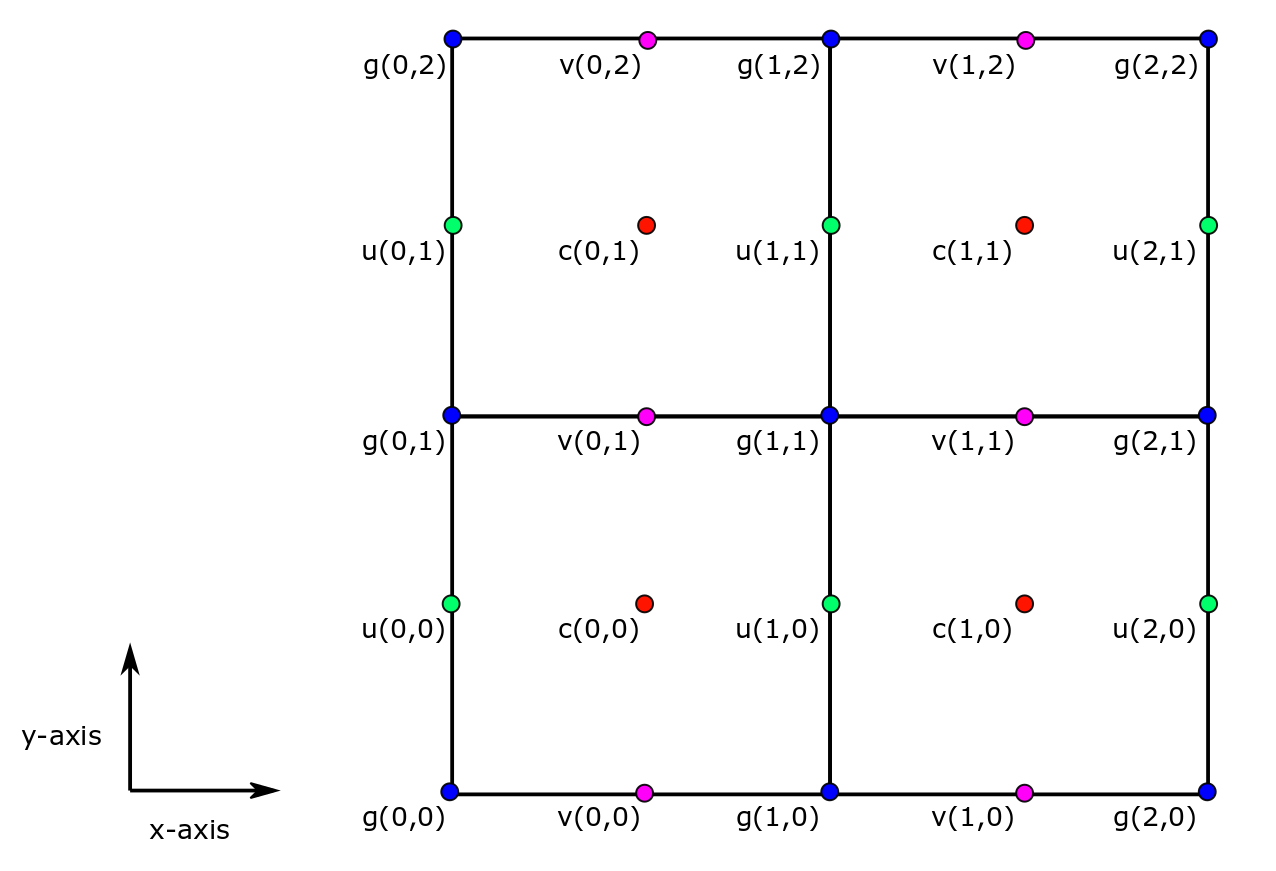
\includegraphics{../figures/C-grid-points.png} \textbf{The four
different classes of points used in the staggered Arakawa-C grid
(C-grid)}

\subsubsection{\texorpdfstring{\emph{c}
points}{c points}}\label{c-points}

Variables that do not have a horizontal velocity component (e.g., T, S,
SSH, OBP, sea ice concentration, vertical velocity) are situated at
\(c\) points in the horizontal plane. \(c\) points are at the center of
the \emph{tracer} grid cell in the horizontal plane.

Let us define the \((i,j)\) coordinate system for the indices of \(c\)
points.

In the ECCO v4 netCDF tile files, \(c(0,0)\) is the -x most and -y most
tracer grid cell.

\begin{itemize}
\tightlist
\item
  In the +\(y\) direction, the next \(c\) point is \(c(0,1)\).
\item
  In the +\(x\) direction, the next \(c\) point is \(c(1,0)\)
\end{itemize}

\subsubsection{\texorpdfstring{\emph{u}
points}{u points}}\label{u-points}

Variables that are explictly related to horizontal velocity or
horizontal fluxes in the model's \(x\) direction are situated at \(u\)
points in the horizontal plane. Examples include horizontal velocity in
the \(x\) direction (\(UVEL\)) and horizontal advective flux of snow in
the \(x\) direction (\(ADVxSNOW\)).

In the \(x\) direction they are situated on the edges or faces of the
tracer grid cell. In the \(y\) direction they are at the same locations
as the \(c\) points.

Let us define the \((i_g, j)\) coordinate system for \(u\) points. We
use \(i_g\) as the coordinate in the \(x\) direction because \(u\)
points are situated along the tracer grid cell ed\textbf{\emph{G}}es. We
use the \(j\) for its \(y\) coordinate because it is the same as the
\(y\) coordinate of the \(c\) points.

In the ECCO v4 netCDF tile files, \(u(0,0)\) is the -x most and -y most
\(u\) point.

\subsubsection{\texorpdfstring{\emph{v}
points}{v points}}\label{v-points}

Variables that are explictly related to horizontal velocity or
horizontal fluxes in the model's \(y\) direction are situated at \(v\)
points in the horizontal plane. Examples include horizontal velocity in
the \(y\) direction (\(VVEL\)) and horizontal advective flux of snow in
the \(y\) direction (\(ADVySNOW\)).

In the \(x\) direction they are at the same locations as the \(c\)
points. In the \(y\) direction they are situated on the edges (or faces)
of the tracer grid cell.

Let us define the \((i, j_g)\) coordinate system for \(v\) points. We
use the \(i\) for its \(x\) coordinate because it is the same as the
\(x\) coordinate of the \(c\) points. We use \(j_g\) as the coordinate
in the \(y\) direction because \(v\) points are situated along the
tracer grid cell ed\textbf{\emph{G}}es.

In the ECCO v4 netCDF tile files, \(v(0,0)\) is the -x most and -y most
\(v\) point.

\subsubsection{\texorpdfstring{\emph{g}
points}{g points}}\label{g-points}

Variables that are explictly related to horizontal velocities in the
model in both the \(x\) and \(y\) direction are situated at \(g\) points
in the horizontal plane. Vorticity is an example.

\(g\) points are situated along the edges of the grid cell in both \(x\)
and \(y\). In other words, they are at the \textbf{corners} of tracer
grid cells.

Let us define the \((i_g, j_g)\) coordinate system for \(g\) points
following the same reasoning as described above: in both the \(x\) and
\(y\) directions, \(g\) points are on the ed\textbf{\emph{G}}es of
tracer grid cells.

In the ECCO v4 netCDF tile files, \(g(0,0)\) is the -x most and -y most
\(g\) point.

\subsection{The two vertical points of the Arakawa-C
gird}\label{the-two-vertical-points-of-the-arakawa-c-gird}

There are two coordinates in the vertical \(z\) dimension:

\subsubsection{\texorpdfstring{\emph{w}
points}{w points}}\label{w-points}

Variables related to vertical velocity or vertical fluxes are situated
at \(w\) in the vertical direction. These variables are situated on the
upper and lower faces of the tracer grid cell.

Let us define the \(k_g\) coordinate system for \(w\) points by
following the same reasoning as we used above: \(w\) points fall along
the the ed\textbf{\emph{G}}es of tracer grid cells in the \(z\)
direction.

Indexing begins at the sea surface, k\_g=0.

\subsubsection{\texorpdfstring{\emph{k}
points}{k points}}\label{k-points}

Let us define \(k\) as the vertical coordinate corresponding with the
middle of a tracer grid cell in the \(z\) direction. All tracers are
situated at \(k\) in the vertical.

Indexing begins in the uppermost grid cell surface, k=0.

\subsection{Applying the C-grid coordinates to the
variables}\label{applying-the-c-grid-coordinates-to-the-variables}

The default coordinate names in the ECCO v4 netcdf tile files do not
distinguish distinguish between the four horizontal coordinates,
\(i, i_g, j, j_g\) and the two vertical coordinates, \(k_w\) and \(k\),
used by the C-grid .

To apply these more descriptive coordinates to the \texttt{Dataset}
objects that are created when we load netCDF files, we have written a
custom routine, \texttt{load\_tile\_from\_netcdf}.

\subsubsection{\texorpdfstring{\texttt{load\_tile\_from\_netcdf}}{load\_tile\_from\_netcdf}}\label{load_tile_from_netcdf}

This routine takes four arguments, 1. \emph{data\_dir}: the directory of
the netCDF file 2. \emph{var}: the name of the netCDF file without the
tile number. 3. \emph{var\_type}: one of 'c','g','u','v', or 'grid'
corresponding with the variables C-grid point type. 'grid' is a special
case because \textbf{GRID} ECCO v4 tile files are unique in that they
contain a mix of 'c','g','u','v','k', and 'w' points. 4.
\emph{tile\_index}: the tile number {[}1 .. 13{]}

    \subsubsection{\texorpdfstring{Loading an ECCO v4 netCDF tile file using
\texttt{load\_tile\_from\_netcdf}}{Loading an ECCO v4 netCDF tile file using load\_tile\_from\_netcdf}}\label{loading-an-ecco-v4-netcdf-tile-file-using-load_tile_from_netcdf}

Let's once again open the grid file for \emph{tile 3} (North East
Atlantic Ocean) using \texttt{load\_tile\_from\_netcdf}

    \begin{Verbatim}[commandchars=\\\{\}]
{\color{incolor}In [{\color{incolor}47}]:} \PY{n}{data\PYZus{}dir}\PY{o}{=}\PY{l+s+s1}{\PYZsq{}}\PY{l+s+s1}{/Volumes/ECCO\PYZus{}BASE/ECCO\PYZus{}v4r3/nctiles\PYZus{}grid/}\PY{l+s+s1}{\PYZsq{}}    
         \PY{n}{var} \PY{o}{=} \PY{l+s+s1}{\PYZsq{}}\PY{l+s+s1}{GRID}\PY{l+s+s1}{\PYZsq{}}
         \PY{n}{var\PYZus{}type} \PY{o}{=} \PY{l+s+s1}{\PYZsq{}}\PY{l+s+s1}{grid}\PY{l+s+s1}{\PYZsq{}}
         \PY{n}{tile\PYZus{}index} \PY{o}{=} \PY{l+m+mi}{3}
         \PY{n}{grid\PYZus{}3\PYZus{}new} \PY{o}{=} \PY{n}{ecco}\PY{o}{.}\PY{n}{load\PYZus{}tile\PYZus{}from\PYZus{}netcdf}\PY{p}{(}\PY{n}{data\PYZus{}dir}\PY{p}{,} 
                                                  \PY{n}{var}\PY{p}{,} 
                                                  \PY{n}{var\PYZus{}type}\PY{p}{,} 
                                                  \PY{n}{tile\PYZus{}index}\PY{p}{)}
\end{Verbatim}


    \begin{Verbatim}[commandchars=\\\{\}]
loading /Volumes/ECCO\_BASE/ECCO\_v4r3/nctiles\_grid/GRID.0003.nc

    \end{Verbatim}

    \begin{Verbatim}[commandchars=\\\{\}]
{\color{incolor}In [{\color{incolor}49}]:} \PY{n}{grid\PYZus{}3\PYZus{}new}
\end{Verbatim}


\begin{Verbatim}[commandchars=\\\{\}]
{\color{outcolor}Out[{\color{outcolor}49}]:} <xarray.Dataset>
         Dimensions:  (i: 90, i\_g: 90, j: 90, j\_g: 90, k: 50, k\_l: 50, k\_u: 50)
         Coordinates:
             tile     int64 3
           * k        (k) float64 1.0 2.0 3.0 4.0 5.0 6.0 7.0 8.0 9.0 10.0 11.0 12.0 {\ldots}
           * i        (i) float64 1.0 2.0 3.0 4.0 5.0 6.0 7.0 8.0 9.0 10.0 11.0 12.0 {\ldots}
           * j        (j) float64 1.0 2.0 3.0 4.0 5.0 6.0 7.0 8.0 9.0 10.0 11.0 12.0 {\ldots}
           * i\_g      (i\_g) float64 1.0 2.0 3.0 4.0 5.0 6.0 7.0 8.0 9.0 10.0 11.0 {\ldots}
           * j\_g      (j\_g) float64 1.0 2.0 3.0 4.0 5.0 6.0 7.0 8.0 9.0 10.0 11.0 {\ldots}
           * k\_u      (k\_u) float64 1.0 2.0 3.0 4.0 5.0 6.0 7.0 8.0 9.0 10.0 11.0 {\ldots}
           * k\_l      (k\_l) int64 1 2 3 4 5 6 7 8 9 10 11 12 13 14 15 16 17 18 19 20 {\ldots}
         Data variables:
             XC       (j, i) float64 {\ldots}
             YC       (j, i) float64 {\ldots}
             RAC      (j, i) float64 {\ldots}
             Depth    (j, i) float64 {\ldots}
             AngleCS  (j, i) float64 {\ldots}
             AngleSN  (j, i) float64 {\ldots}
             hFacC    (k, j, i) float64 {\ldots}
             land\_c   (k, j, i) float64 1.0 1.0 1.0 1.0 1.0 1.0 1.0 1.0 1.0 1.0 1.0 {\ldots}
             XG       (j\_g, i\_g) float64 {\ldots}
             YG       (j\_g, i\_g) float64 {\ldots}
             RAZ      (j\_g, i\_g) float64 {\ldots}
             DXC      (j, i\_g) float64 {\ldots}
             DYG      (j, i\_g) float64 {\ldots}
             hFacW    (k, j, i\_g) float64 {\ldots}
             land\_u   (k, j, i\_g) float64 1.0 1.0 1.0 1.0 1.0 1.0 1.0 1.0 1.0 1.0 1.0 {\ldots}
             DYC      (j\_g, i) float64 {\ldots}
             DXG      (j\_g, i) float64 {\ldots}
             hFacS    (k, j\_g, i) float64 {\ldots}
             land\_v   (k, j\_g, i) float64 1.0 1.0 1.0 1.0 1.0 1.0 1.0 1.0 1.0 1.0 1.0 {\ldots}
             RF       (k\_u) float64 {\ldots}
             DRC      (k\_u) float64 {\ldots}
             RC       (k) float64 {\ldots}
             DRF      (k) float64 {\ldots}
             RB       (k\_l) float64 -10.0 -20.0 -30.0 -40.0 -50.0 -60.0 -70.0 -80.01 {\ldots}
         Attributes:
             description:    C-grid parameters (see MITgcm documentation for details){\ldots}
             A:              :Format      = native grid (nctiles w. 13 tiles)
             B:              :source      = ECCO consortium (http://ecco-group.org/)
             C:              :institution = JPL/UT/MIT/AER
             D:              :history     = files revision history :
             E:                                 04/20/2017: fill in geometry info for {\ldots}
             F:                                 11/06/2016: third release of ECCO v4 ({\ldots}
             G:                             estimates revision history (from second re{\ldots}
             H:                                 employs bi-harmonic viscosity (enhance{\ldots}
             I:                                 sea-ice parameters, updated or novel o{\ldots}
             J:                                 GRACE OBP, Aquarius SSS, global mean s{\ldots}
             K:                                 time-series, extended and/or expanded {\ldots}
             L:                                 revised weights including data and con{\ldots}
             M:                                 to account for grid-size variation and{\ldots}
             N:                                 separate time-mean and time-variable d{\ldots}
             O:                                 and controls, sea-ice costs, and initi{\ldots}
             P:                                 additional controls.\textbackslash{}n 
             Q:              :references  = Forget, G., J.-M. Campin, P. Heimbach, C. {\ldots}
             R:                              and C. Wunsch, 2015: ECCO version 4: an i{\ldots}
             S:                              non-linear inverse modeling and global oc{\ldots}
             T:                              Geoscientific Model Development, 8, 3071-{\ldots}
             U:                             Forget, G., J.-M. Campin, P. Heimbach, C. {\ldots}
             V:                              ECCO version 4: Second Release, 2016, htt{\ldots}
             W:              file created using gcmfaces\_IO/write2nctiles.m
             date:           21-Apr-2017
             Conventions:    CF-1.6
             \_FillValue:     nan
             missing\_value:  nan
\end{Verbatim}
            

    % Add a bibliography block to the postdoc
    
    
    
    \end{document}
